% LaTex Klasse
\documentclass[11pt,a4paper,article,oneside]{memoir}

%% Pakete default
\usepackage[utf8]{inputenc} 
\usepackage[backend=biber,bibencoding=utf8,sorting=nyt,language=ngerman, style=alphabetic]{biblatex}
\usepackage[breaklinks=true]{hyperref}
\usepackage[german]{babel}
\usepackage{graphicx}
\usepackage{subfloat}
\usepackage{eurosym}
\usepackage{amsmath}

%% Pakete usefull
\usepackage{tikz}
%\usepackage{tikzscale}
%\usepackage{bbding}
%\usepackage{listings} 
%\usepackage{epstopdf}
%\usepackage{pgfgantt}
%\usepackage{wrapfig}
%\usepackage{mathtools}
%\usepackage[page]{appendix}

%% R\"omishce zeichen
%\newcommand{\rmnum}[1]{\romannumeral #1}

%%line space
\DisemulatePackage{setspace}
\usepackage{setspace}
%%set global linespace
\newcommand{\mylinespace}{1.1}

% Image floating
%\newcommand{\illustrationname}{Illustration}
%\newfloat[chapter]{illustration}{lol}{\illustrationname}

%% Absatzeinzug!!!
\setlength{\parindent}{0pt}

%% TiKz Stuff %%%
\usetikzlibrary{calc, decorations.pathmorphing,decorations.pathreplacing, fadings, shadings, shapes, arrows,trees, positioning,patterns,automata}
%\pgfdeclarelayer{background}
%\pgfdeclarelayer{foreground}
%\pgfsetlayers{background,main,foreground}
%\usepackage{tikz-uml}
%\usepackage{pgfplots}

%% Bib
%\bibliography{references}
%\defbibheading{bibliography}{\bibsection}


%% PAGE DIMENSIONS A4  % This is from memman.pdf
\settrimmedsize{297mm}{210mm}{*}
\setlength{\trimtop}{0pt}
\setlength{\trimedge}{\stockwidth}
\addtolength{\trimedge}{-\paperwidth}
\settypeblocksize{670pt}{410pt}{*}
\setulmargins{3cm}{*}{*}
\setlrmargins{*}{*}{0.8}
\setmarginnotes{17pt}{51pt}{\onelineskip}
\setheadfoot{\onelineskip}{2\onelineskip}
\setheaderspaces{*}{2\onelineskip}{*}
\checkandfixthelayout

%\maketitle % CUSTOMISATION
 % to be done
 %\pagenumbering{Roman}

% For more than trivial changes, you may as well do it yourself in a titlepage environment 
 %\pretitle{\begin{center}\sffamily\huge\MakeUppercase}
 %\posttitle{\par\end{center}\vskip 0.5em}

%%% ToC (table of contents) APPEARANCE
 %\maxtocdepth{subsection} % include subsections
 %\renewcommand{\cftchapterpagefont}{}
 %\renewcommand{\cftchapterfont}{} % no bold!

%%% HEADERS & FOOTERS
\pagestyle{plain} % try also: empty , plain , headings , ruled , Ruled , companion

%%% CHAPTERS
\chapterstyle{section} %southall} % try also: default , section , hangnum , companion , article, demo

\renewcommand{\chaptitlefont}{\Huge\sffamily\raggedright} % set sans serif chapter title font
\renewcommand{\chapnumfont}{\Huge\sffamily\raggedright} % set sans serif chapter number font

%%% SECTIONS
%\hangsecnum % hang the section numbers into the margin to match \chapterstyle{hangnum}
\maxsecnumdepth{subsection} % number subsections

\setsecheadstyle{\Large\sffamily\raggedright} % set sans serif section font
\setsubsecheadstyle{\large\sffamily\raggedright} % set sans serif subsection font


%% END Memoir customization

%% TikZ input Hack
 \newcommand{\inputTikZ}[1]{\input{#1.tikz}} 
 %\newsubfloat{figure} %% use for \subbottom or \subtop in a figure

%%%##########################################
% Content Composer
\newboolean{de}
\newboolean{fullfrontpage}


\setboolean{de}{true} %DE - true; EN - false
\setboolean{fullfrontpage}{true} % full - true; just a header - false

%set publisher
\newcommand{\docType}{Lab Report}
\newcommand{\docTypeRubric}{Sandkasten Bla Blub Thema}
\newcommand{\docCourse}{Master Projekt System Entwicklung}
\newcommand{\docCourseSemester}{SS 2013}
\newcommand{\docCourseProf}{Prof. Dr. J. Wietzke, Prof. Dr. E. Hergenroether}
\newcommand{\docDate}{01.05.2013}
\newcommand{\docStudentA}{T. Sturm}
\newcommand{\docStudentAMatrikel}{000000}
\newcommand{\docStudentB}{A. Holike}
\newcommand{\docStudentBMatrikel}{724986}
\newcommand{\docStudentC}{S. Arthur}
\newcommand{\docStudentCMatrikel}{000000}
\newcommand{\docStudentD}{M. Djakow}
\newcommand{\docStudentDMatrikel}{000000}

%%% #########################################
%%% BEGIN DOCUMENT

\begin{document}

%Titel
\iffullfrontpage
	% !TEX root = ../report.tex
% begin title
\begin{titlingpage}
	\vspace*{0cm}
	\sffamily 
	\begin{centering}
		
\includegraphics[width=0.5\textwidth]{images/fbi_logo.pdf} \\
		\vspace{2.5cm}
		\Huge
			\textbf{\docType} \\
		\vspace{1cm}
		\normalsize
			\docCourse, \docCourseSemester \\
		\small
			(\textit{\docCourseProf}) \\
		\vspace{3cm}
		\LARGE
			\docTypeRubric \\
		\vspace{5cm}
		\normalsize
			\ifde
				vorgelegt von\\
			\else
				submitted by\\
			\fi
		\vspace{1cm}	
		\large
			\docStudentA \hspace{0.1cm} (\docStudentAMatrikel)\\
			\vspace{0.2cm}
			\docStudentB \hspace{0.1cm} (\docStudentBMatrikel)\\
			\vspace{0.2cm}
			\docStudentC \hspace{0.1cm} (\docStudentCMatrikel)\\
			\vspace{0.2cm}
			\docStudentD \hspace{0.1cm} (\docStudentDMatrikel)\\
			\vspace{1cm}
		\normalsize
			\docDate \\
	\end{centering}
	
\end{titlingpage}

%% End Of Doc
\else
	% !TEX root = ../report.tex
% begin title
\begin{centering}
	\sffamily
	\vspace*{0.5cm}
	\huge
		\docType \\
	\vspace{0.5cm}
	\small
		\docCourse, \docCourseSemester \\
	\footnotesize
		(\textit{\docCourseProf}) \\
	\vspace{0.5cm}
		\large
			\docTypeRubric, \hspace{0.1cm} \docDate \\
		\vspace{0.5cm}
		\small
			\ifde
				vorgelegt von\\
			\else
				submitted by\\
			\fi
		\vspace{0.25cm}	
		\small
			\docStudentA \hspace{0.1cm} (\docStudentAMatrikel)\\
			\docStudentB  \hspace{0.1cm} (\docStudentBMatrikel)\\
		\vspace{0.5cm}
		
		\rule{12cm}{0.025cm}
		
\end{centering}
\vspace{1cm}
%% End Of Doc
\fi

\tableofcontents* % the asterisk means that the contents itself isn't put into the ToC

\clearpage %schreibt letztes Kapitel fertig, noetig fuer toc


%%% BEGIN  CONTENT %%%
%% Styles für TikZ
  %\include{graphics/styles}

% !TEX root = ../report.tex
\chapter{Einleitung}
\begin{Spacing}{\mylinespace}
\begin{figure}[h!]
	\centering
	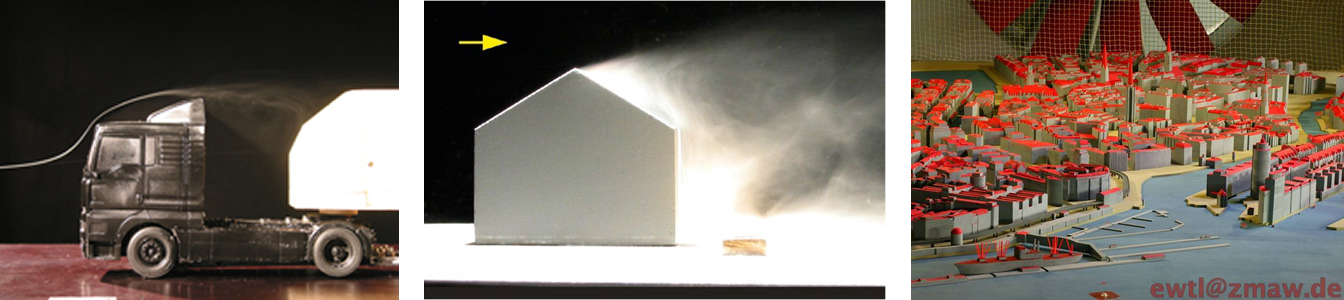
\includegraphics[width=\textwidth]{graphics/intro.png}
\end{figure}
Die Technik der Strömungssimulation spielt heutzutage eine größere Rolle den je. Lange ist es her das Windkanäle nur zur Erforschung und Verbesserung der Aerodynamik von Flugzeugen genutzt wurde. Heute gibt es kaum noch ein Kraftfahrzeug das nicht im Windkanal optimiert wurde und auch Architekten und Statiker nutzen immer häufiger den Windkanal um ihre Konstruktionen und Berechnungen zu überprüfen. Ein relativ neues Thema in diesem Gebiet ist die Untersuchung kompletter Stadtteilen und Städten im Windkanal. Durch den enormen Anstieg von neuen Wohn-, Gewerbe- und Industriegebieten in den letzten Jahrzehnten, schrumpft der Anteil von freien und natürlichen Flächen immer weiter, wodurch die Frischluftzufuhr negativ beeinflusst wird und sich das Klima in Städten stetig weiter erwärmt und verschlechtert. Um dieser Entwicklung entgegen zu wirken nutzen auch Städteplaner immer häufiger die Vorzüge des Windkanals.
\\\\
So nützlich der Windkanal auch für alle vorgestellten Anwendungen ist, so ist dessen Nutzung auch immer mit sehr hohen Kosten verbunden. Durch die immer weiter steigende Leistung von Computern liegt es deshalb nahe, zu versuchen, erste Tests und Untersuchung von der Realität auf den Computer auszulagern und auf diesem zu simulieren. Genau aus diesem Gebiet bestand der Hauptteil unserer Forschung in diesem Semester. Um dieses doch sehr mathematische und trockene Thema für Außenstehende noch etwas attraktiver und greifbarer zu machen haben wir es jedoch, mit Hilfe der Kinect Kamera von Microsoft, noch um eine Interaktive Komponente erweitert.
\\\\
Auf den Folgenden Seiten werden wir nun unser Vorgehen sowie die Fortschritte, Erfahrungen und Ergebnisse dieses Projekts vorstellen.
\end{Spacing}
\newpage
\clearpage
%% End Of Doc
\clearpage
% !TEX root = ../report.tex
\chapter{Bestehende Arbeiten}
\begin{Spacing}{\mylinespace}
\begin{figure}[h!]
	\centering
	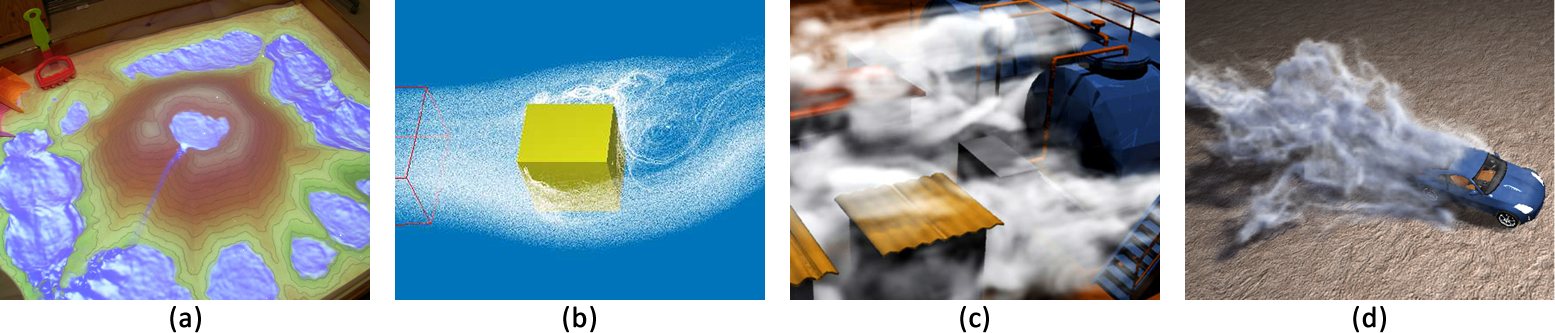
\includegraphics[width=\textwidth]{graphics/relatedWork.png}
	\caption{(a) Augmented Reality Sandbox. (b) A Particle System
for Interactive Visualization of 3D Flows. (c) Synthetic Turbulence using Artificial Boundary Layers. (d) Scalable Fluid Simulation using Anisotropic Turbulence Particles}
	\label{fig:relatedWork}
\end{figure}
Bevor wir auf unsere eigene Arbeit eingehen, wollen wir kurz einige andere Arbeiten vorstellen die sich mit ähnlichen Themen beschäftigen und an denen wir uns zum Teil orientiert haben.
\\\\
Beginnen wollen wir mit der \textit{Augmented Reality Sandbox} \cite{Kreylos2010} einem beeindruckenden Projekt der \textit{University of California} in Zusammenarbeit mit weiteren Forschungsinstituten, welches die Grundidee zu unserer Integrierung der Kinect 3D Kamera von Microsoft und dem Sandkasten lieferte. Ziel dieses Projekts war es, mit Hilfe der Kinect Kamera, eine spielerische Möglichkeit zu entwickeln, die es erlaubt topologische Landschaft, durch formen des Sandes mit den eigenen Händen, zu erstellen. Zusätzlich nutzen sie auch ein physikalisches System zur Simulation von Wasser die man in Abbildung \ref{fig:relatedWork} gut erkennen kann.
\\\\
Mit physikalischen System in Bezug auf Strömungssimulation beschäftigen sich auch die folgenden Arbeiten. \textit{A Particle System
for Interactive Visualization of 3D Flows} \cite{Krueger2005} ist zwar schon etwas älter, aber es ist eine der ersten Arbeiten in der mit der Auslagerung der Physikberechnung auf die GPU, um realistische Echtzeitströmungen zu simulieren, experimentiert wird. Zudem werden sehr interessante Konzepte nutzt, wie zum Beispiel die Speicherung der Partikelpositionen in einer Textur die gleichzeitig als Ein- und Ausgabecontainer zwischen den einzelnen Berechnungsschritten dient.
\\\\
Eine weitere interessante Arbeit ist \textit{Synthetic Turbulence using Artificial Boundary Layers} \cite{Pfaff2009}. Hier werden vorberechnete Strömungsfelder zur Simulation der Partikel genutzt umso extrem realistische Darstellungen zu realisieren. Durch die Vorberechnung verfügt dieses Verfahren aber leider über keine Echtzeitfähigkeit. In der Folgearbeit \textit{Scalable Fluid Simulation using Anisotropic Turbulence Particles} \cite{Pfaff2010} wird dieses Manko, durch starke Parallelisierung und der Berechnung vieler kleineren Einzelsimulationen, allerdings behoben.



\end{Spacing}
\newpage
\clearpage
%% End Of Doc
\clearpage
% !TEX root = ../report.tex
\chapter{Konzept}
\begin{Spacing}{\mylinespace}

wie sieht unser konzept aus\\

\end{Spacing}
\newpage
\clearpage
%% End Of Doc
\clearpage
% !TEX root = ../report.tex
\chapter{Grundlagen}
\begin{Spacing}{\mylinespace}

Hier kommt immer die Kapitelüberschrift hin, ein kleines Vorgeplänkel was im Kapitel behandelt wird.

\section{Mathematische Verfahren}

\subsection{Verzerrung von Bildern}

\subsection{Billboarding}

Um unsere Vorgabe der Echtzeitfähigkeit zu erfüllen benötigt es ein paar Tricks, die es erlauben die Komplexität unseres Renderers zu minimieren, gleichzeitig jedoch darf dem Zuschauer diese Manipulation nicht bemerken.
Eine beliebte Technik hierfür ist das Billboarding. Die Idee des Billboardings basiert darauf, komplexe geometrische 3D-Objekte auf ein zweidimensionales Rechteck das sogenannte Billboard runterzubrechen. 
Bei dem Billboard handelt es sich meist um ein vorher berechnetes Bild von dem ursprünglich darzustellenden 3D-Objekts.
Anschließend wird dieses Billboard zur Kamera ausgerichtet, dem Zuschauer fällt es somit sehr schwer zu erkennen, das es sich bei dem gezeigten Objekt um eine zweidimensionale Kopie des 3D-Objektes handelt.
Diese Technik wird hauptsächlich dazu verwendet die benötigten Rechenoperationen für Objekte welche in der Ferne liegen zu minimieren. 
Kommt die Kamera dem tatsächlichen Objekten sehr nahe, wird meist mit einer Interpolation zwischen dem Billboard und dem tatsächlichen 3D-Objekt umgeschaltet.
\end{Spacing}
\newpage
\clearpage
%% End Of Doc
\clearpage
% !TEX root = ../report.tex
\chapter{Kinect Integration}
\begin{Spacing}{\mylinespace}

hier wird die dll erklärt und wie sie eingebunden wird\\
kinect baut metrik vom bild um veraenderungen wahrzunehmen\\
sendet event nur wenn neues Tiefenbild vorhanden\\
tiefenbild blur\\

\end{Spacing}
\newpage
\clearpage
%% End Of Doc
\clearpage
% !TEX root = ../report.tex
\chapter{XNA Renderer}
\begin{Spacing}{\mylinespace}

wie tut der renderer \\
warum haben wir den genommen\\
vorteile\\


\end{Spacing}
\newpage
\clearpage
%% End Of Doc
\clearpage
% !TEX root = ../report.tex
\section{Partikelsystem}
\begin{Spacing}{\mylinespace}

Es gibt verschiedene Möglichkeiten ein Partikelsystem zu realisieren.
In unserem Anwendungsfall haben wir uns dafür entschieden Visualisierung und Physik zu trennen.
Dies führt dazu, das es möglich ist, ohne große Abhängigkeiten voneinander parallel zu entwickeln.

\subsection{Die Physik (Physik-Engine)}
Damit die Partikel möglichst realitätsgetreu sich durch die Szene bewegen, benötigt der Computer die Information wie sich die entsprechenden Partikel verhalten sollen.
Dies bedeutet das physikalische Gesetze auf mathematische Funktionen abgebildet werden müssen.
Durch diese Abbildung werden die Bewegungsabläufe der Partikel gesteuert.
Um die Echtzeitfähigkeit des Systems sicher zu stellen müssen meist die Abbildungen (Gesetze) durch ein paar Tricks vereinfacht werden um Rechenkraft zu sparen.

Die Physik-Engine hat genau diese Aufgaben; Sie bewegt die Partikel durch den Raum, erkennt Kollisionen und bildet Gesetzte der \ref{Reflektion} ab.
Durch die hohe Unabhängigkeit von den einzelnen Partikeln eignet sich eine GPU besonders gut zum berechnen entsprechender Gesetze.
Wir haben uns dennoch im aktuellen Projektstatus dazu entschieden die Berechnungen auf der CPU durchzuführen.
Der Grund hierfür liegt in der Problematik das es nicht möglich ist Berechnungen welche auf der GPU stattfinden genauer zu untersuchen bzw. zu Debuggen.

\subsection{Der Renderer (Draw-Engine)}
Der Renderer ist der zweite Teil unseres Partikelsystems. Seine Aufgabe liegt darin, für jedes einzelnes Partikel die Eigenschaften (Farbe,Kraft,Größe,...) für den Benutzer zu visualisieren.
Hierbei wird lediglich lesend auf den vorhandene Datenbestand zugegriffen.
Auch hier ist eine hohe Parallelität möglich, denn jedes Partikel stellt eine unabhängige Einheit dar.
Somit ist es möglich mit Hilfe von DirektX einen Shader für die GPU zu schreiben. 
Dieser erlaubt es, das alle Shader-Units der GPU zusammen an einem Frame arbeiten. 

\end{Spacing}
\newpage
\clearpage
%% End Of Doc
\clearpage
% !TEX root = ../report.tex
\section{GUI}
\begin{Spacing}{\mylinespace}

anbindung der elemente \\
darstellungsart bla blub\\
integration xna in gui etc\\
kallibration der sandkiste\\


\end{Spacing}
\newpage
\clearpage
%% End Of Doc
\clearpage
% !TEX root = ../report.tex
\chapter{Ergebnisse}
\begin{Spacing}{\mylinespace}

hier schreiben wir unsere erfahrungen rein undwas wir genau hinbekommen haben. zudem sollen probleme die währed der arbeit aufgetreten sind erwähnt / erläutert werden. \\

\end{Spacing}
\newpage
\clearpage
%% End Of Doc
\clearpage
% !TEX root = ../report.tex
\chapter{Probleme}
	\section{Echtzeitfähigkeit}
		Leider besitzt die derzeitige Ausarbeitung diverse kleinere Probleme, welche die Echtzeitfähigkeit des Systems gefährden.
		Diverse teile von Berechnungen werden noch wie in \ref{physik} beschrieben auf der CPU ausgeführt, während der Teil der Visualisierung bereits auf die GPU portiert wurde.
		Dies führt zu erheblichen Performanceproblemen, denn es muss bei jeder Physikberechnung (jeden Frame), die Partikeldaten zwischen GPU und CPU kopiert und synchronisiert werden.
	\section{Darstellung}
		Die Darstellung stellte sich um Laufe des Projektes als schwieriger heraus als vorher angedacht.
		Hierbei kann man die Probleme auf welche wir gestoßen sind grob in Hard- und Softwareprobleme unterscheiden.
		\subsection{Hardware}
			Trotz das wir einen Beamer von einem Grafiklabor der Hochschule zur Verfügung gestellt bekommen haben, bemerkten wir bereits bei ersten Tests, das ein großer Farbunterschied zwischen Beamer und
			Monitor vorhanden ist. Leider scheint das Spektrum unseres Beamers sehr begrenzt zu sein, so das wir einen Farbunterschied zwischen weiß und gelb kaum wahrnehmen können.		
		\subsection{Software}
			Durch die physikalische Gegebenheit das Kinekt und Beamer sich an unterschiedlichen Orten befinden, entsteht bei der Projektion zusätzlich zur Verzerrung auch noch das Problem der Verschiebung.
			Die Kalibrierung stellte sich somit schwieriger heraus als bisher gedacht, deshalb wurden aus zeitlichen Gründen der Fokus auf Aufgaben gesetzt um schnellstmöglich eine lauffähige Version zu erstellen.

\chapter{Ausblick}
	\begin{Spacing}{\mylinespace}
	Trotz das auf uns allerlei Probleme zukamen, entstand im Laufe eines Semesters eine Echtzeit Sandkastensimulation, die bereits grundlegende Funktionalität bietet. 
	Im Laufe des nächsten Semesters werden wir dann Aufgaben, welche in diesem Semester ein wenig vernachlässigt wurden wie z. B. die Kalibrierung nachbessern.
	Des Weiteren werden wir die bisherigen Physikberechnungen auf die GPU portieren um so hoffentlich wieder die Echtzeitfähigkeit des Systems zu erlangen.
	Auch neue Funktionalitäten sind geplant, welche notwendig sind um unser eigentliches \ref{Ziel} zu erreichen.
	
\end{Spacing}
\newpage
\clearpage
%% End Of Doc
\clearpage
 %and so on
\inputTikZ{graphics/hardware}
%% end of doc
\clearpage

%\pagenumbering{Alph}

%\newpage
%\printbibliography

%\newpage
%\listoffigures
%\newpage

%%%Anhang
%\appendix
%\renewcommand{\appendixtocname}{Anhang}
%\renewcommand{\appendixpagename}{\textsf{Anhang}}

%\appendixpage

\end{document}
